\chapter{Subways I}

\resp{Tomás Mezquita}


\section{Making the node and edge files}
 
We are working with data from different city subways: Moscow, New York (new and old), Tokyo, Paris, Osaka, Seoul, and Shanghai. Each city has a folder which contains different txt files. In this folders we can find:

\begin{itemize}
    \item \textbf{Topologies folder}: containing the networks of all the years since the subway is active. I did not use these files.
    \item \textbf{Line files}: Containing two columns with the name of the line's start and end station. One of the files also contains all the lines and the year that started. These files are important to create the edge file.
    \item \textbf{Station Position Years (SPY) file}: contains the name, latitude and longitude, and year of inauguration of each station. This file is important to make the node list.
\end{itemize}
    
There are also some of the cities folders containing old versions of its subway data. 

To process this data I am using R language using read.table to read the files and different functions to do the processing.


For the node file, it was pretty straightforward, using the SPY file, I just had to add the nodeID to the columns. The only problem that I encountered is that in some files there were more than one year. My guess, is that the first one is the date of the inauguration and the following ones could be renovations of the station, so I took the first four columns of the file as they contain the information that I wanted to save. I obtained the node file for each city selecting the paths of each city using list.files to select the pattern of the paths to the SPY file (which can be different), and grep to discard some of the files that don't contain relevant information.


Creating the edge file was more challenging, I used dplyr library to take advantage of relational databases. To ensure that the nodeID is the same as in the node file I created a lookup table where the nodeID and nodeLabel (name of the station) are stored. Moreover, I have to process the line files and change them from the names of the start and end stations to the nodeID of each station using the lookup table. I also have to process the lines file to obtain the line name and year. 

Having these support functions, we can create the principal function which creates an edge file for a given city, we will need primarily, as inputs the node file, line files, and the lines file where the years are stored. The line paths have approximately the following structure: "data/City/city-lineN.txt" and using list.files we want to extract the line name ("lineN") then we run our secondary functions to obtain the different data and for each subway line path we obtain the year comparing the line name obtained from the path and the lines file, later we put the start and final nodeID, line and year of each edge into the edge file.

The second challenge of this task is to select the file paths for each city and ensure that the line name obtained from the path is the same as in the lines file. The problem is that some city path structures are different, so I had to add some controls for some cities to extract the correct line name. After addressing this issues, I successfully created the edge files as required.


\section{Analysis of the networks}

With the nodes and edges files in hand, we can easily reconstruct the graph using the "graph\_from\_data\_frame" function from the "igraph" library. Here is the visualization of all the 8 cities subway graphs. For clarity, I have set the lines of the subways in different colors. Here are the results:


% Create a figure environment
\begin{figure}[!htb]
    \centering % Center all images
    % Row 1
    \begin{minipage}[b]{0.24\textwidth} % Width of each image
        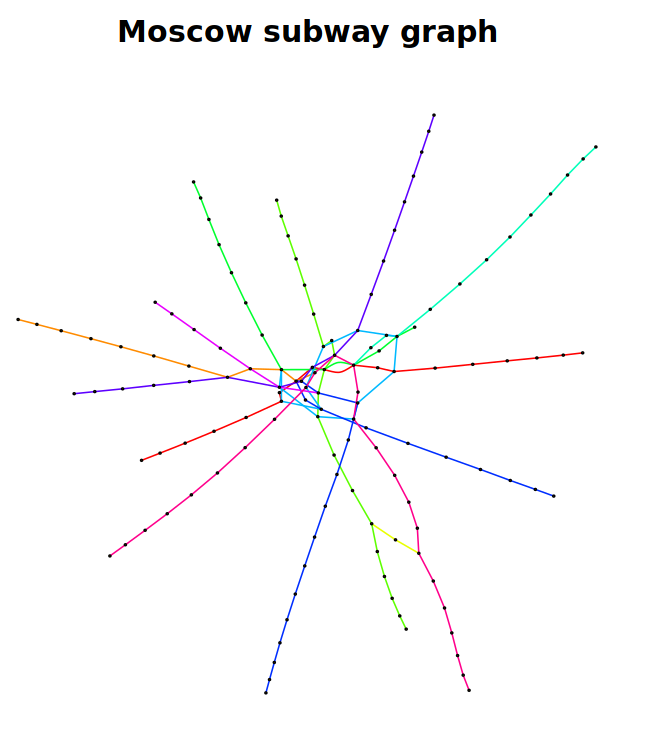
\includegraphics[width=\textwidth]{images/CityGraph_Moscow.png}

    \end{minipage}
    \hfill % Horizontal spacing
    \begin{minipage}[b]{0.24\textwidth}
        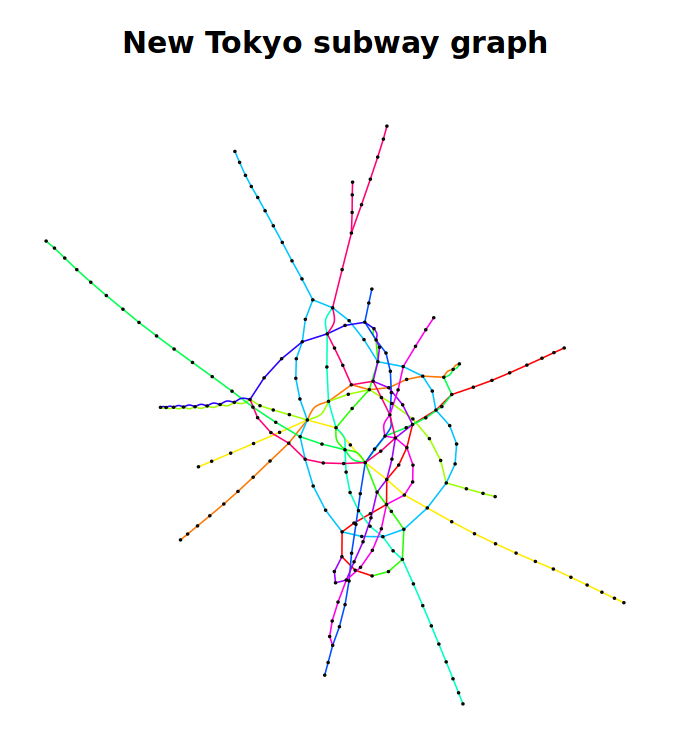
\includegraphics[width=\textwidth]{images/CityGraph_New Tokyo.png}

    \end{minipage}
    \hfill
    \begin{minipage}[b]{0.24\textwidth}
        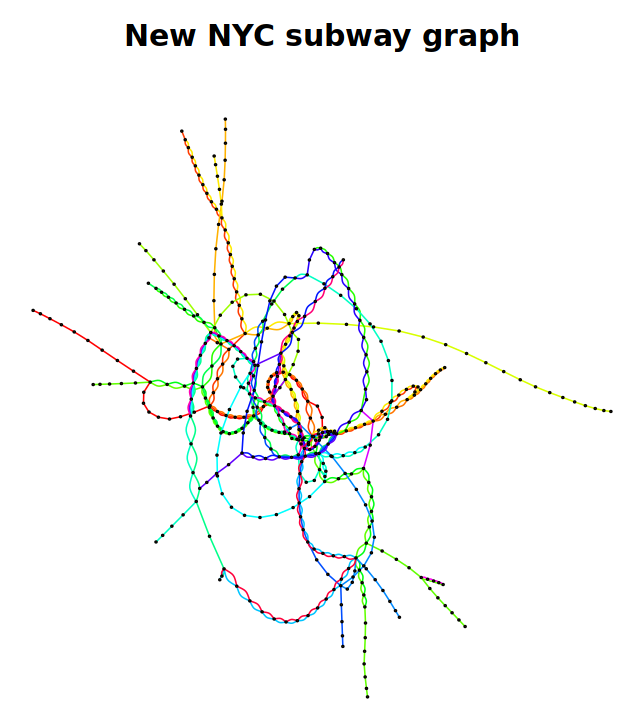
\includegraphics[width=\textwidth]{images/CityGraph_New NYC.png}

    \end{minipage}
    \hfill
    \begin{minipage}[b]{0.24\textwidth}
        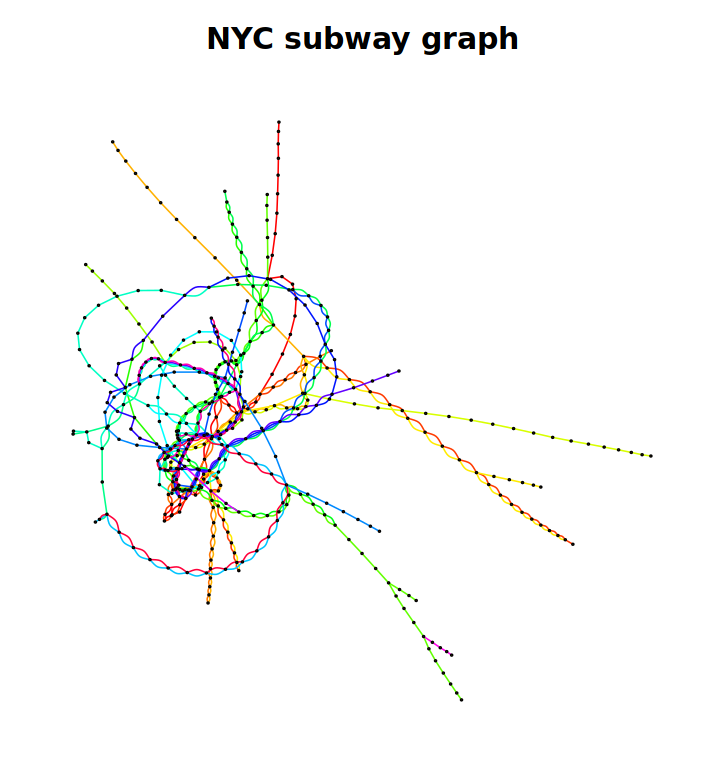
\includegraphics[width=\textwidth]{images/CityGraph_NYC.png}

    \end{minipage}
    
    \vspace{0cm} % Vertical space between rows

    % Row 2
    \begin{minipage}[b]{0.24\textwidth}
        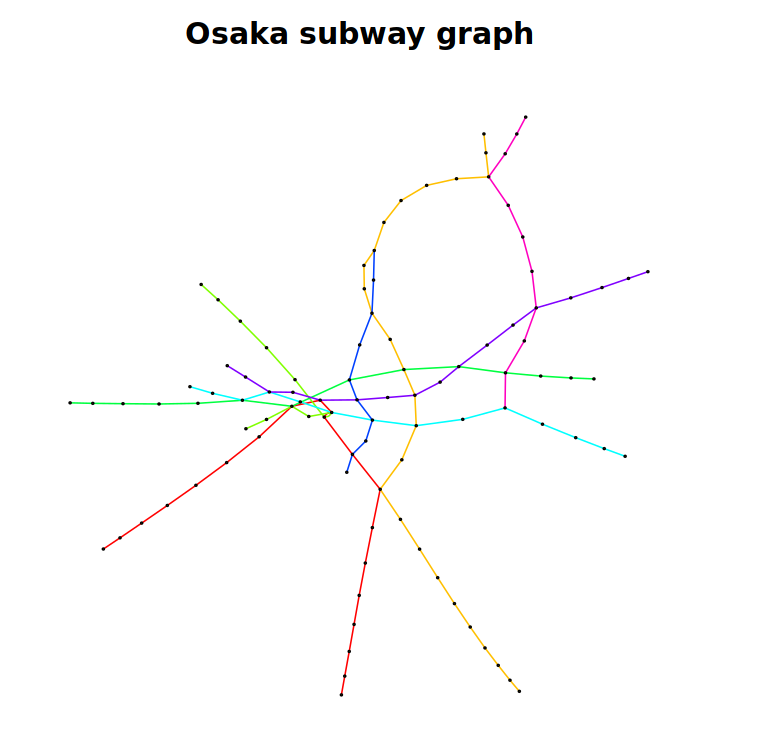
\includegraphics[width=\textwidth]{images/CityGraph_Osaka.png}
 
    \end{minipage}
    \hfill
    \begin{minipage}[b]{0.24\textwidth}
        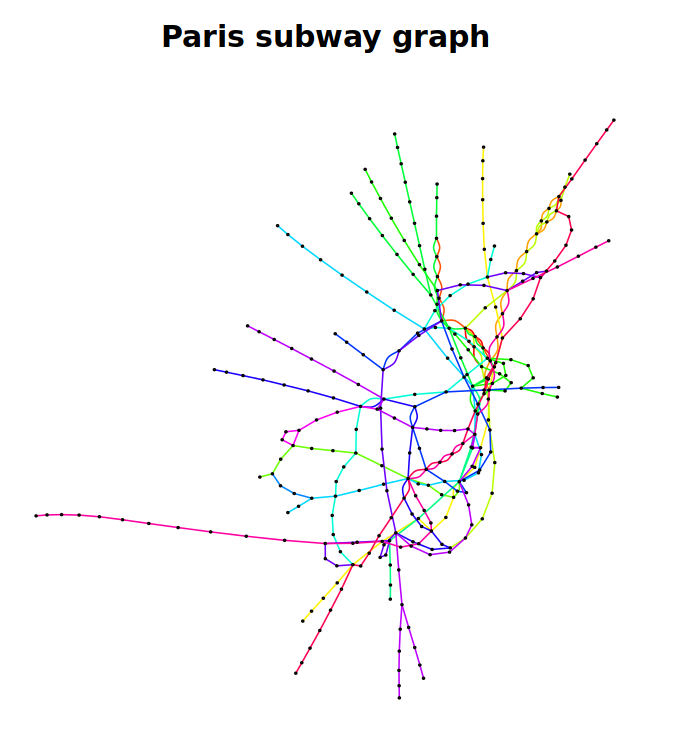
\includegraphics[width=\textwidth]{images/CityGraph_Paris.png}

    \end{minipage}
    \hfill
    \begin{minipage}[b]{0.24\textwidth}
        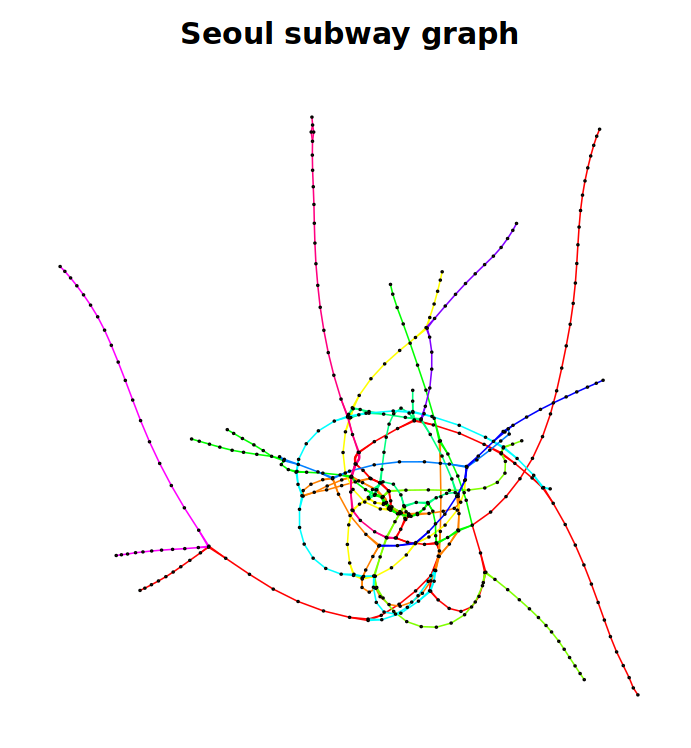
\includegraphics[width=\textwidth]{images/CityGraph_Seoul.png}

    \end{minipage}
    \hfill
    \begin{minipage}[b]{0.24\textwidth}
        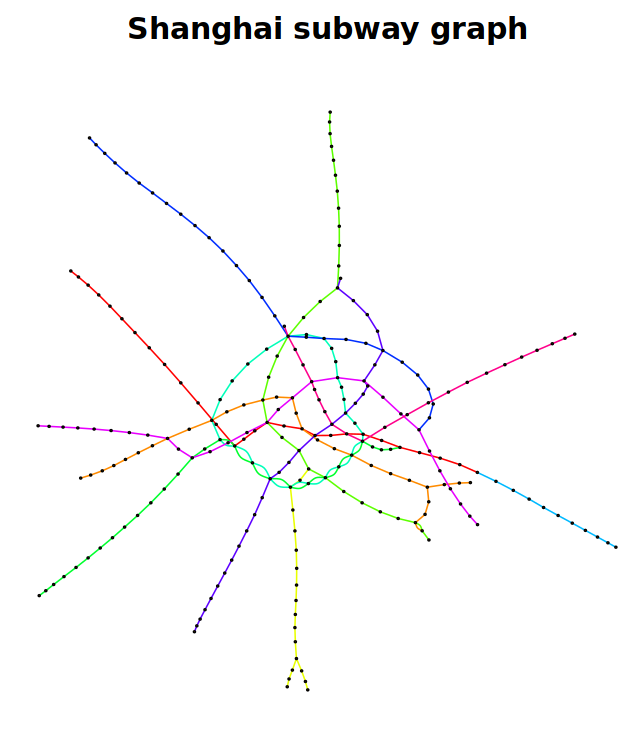
\includegraphics[width=\textwidth]{images/CityGraph_Shanghai.png}

    \end{minipage}

\end{figure}


As observed, all the cities exhibit a similar pattern: a central area that is more connected, representing the city center, where most of the lines pass through and nodes have a higher degree, or in other words, where the stations are more likely to connect with other lines. Otherwise, the outer regions of the graph display lines that are less connected with other lines. We observe a representative case of this phenomenon in the Moscow graph, where the external lines are rarely connected. This is due to these lines extending into the outskirts of the city, moving away from the city center and becoming more isolated from other lines. 

This pattern makes sense, as city centers have higher population densities and more activity so the transportation requirements are higher.  Contrarily, the outskirts of a city experience less activity and the requirements are lower, with more routes converging towards the city center. It would be interesting to study a multilayer network that combines the population density with vatious transportation networks for a better understanding of these dynamics.


Next, we will analyze the graphs quantitatively by computing some quantities that will help us with a better understanding of the nature of the graphs and its characteristics. These metrics include mean degree, cluster coefficient,  average length path, size of the connected component, etc. I have summarized these magnitudes in the table below:

\begin{table}[h]
\centering
\footnotesize
\begin{tabular}{|l|r|r|r|r|r|}
\hline
\textbf{City} & \textbf{Mean Degree} & \textbf{Diameter} & \textbf{Avg. Path Length} & \textbf{Cluster Coef.} & \textbf{Assortativity} \\ \hline
Moscow        & 2.343284             & 24                & 9.440579                    & 0.019608                        & 0.465932               \\ 
New Tokyo     & 2.562212             & 32                & 10.398916                   & 0.025428                        & 0.253371               \\ 
New NYC       & 4.322581             & 59                & 20.989421                   & 0.018070                        & 0.371283               \\ 
NYC           & 3.958525             & 55                & 16.114228                   & 0.029114                        & 0.319052               \\ 
Osaka         & 2.300000             & 23                & 8.454545                    & 0.000000                        & 0.209897               \\ 
Paris         & 2.664452             & 33                & 11.793289                   & 0.022405                        & 0.200149               \\ 
Seoul         & 3.141667             & 66                & 19.912804                   & 0.008336                        & 0.760314               \\ 
Shanghai      & 2.292887             & 41                & 14.577160                   & 0.001943                        & 0.175337               \\ \hline
\end{tabular}
\end{table}

From these magnitudes, we can extract significant information on the network structures. For instance, both the New York (both new and old systems) and Seoul subways show high mean degrees (3-4), large diameter of the GCC (40-60), high average path length (15-20), and high assortativity (0,3-0,7). 

This metrics suggest dense, large, and more connected graphs. In practical terms, this means they have a more developed structure with more interconnected stations making them more navigable. High assortativity shows that stations with similar connectivity levels are likely to be connected, indicating a hierarchical structure where major stations are more likely to connect with other hubs.

In contrast, Moscow, Osaka, and Shanghai have a simpler structur with lower magnitudes compared to the previous ones: low mean degree (around 2,3), diameter (20-25), and average path length (8-10). Seoul seems to have a bigger subway structure as it has a higher diameter (41) and average length path (14,58). This type of networks traduce into a simpler subway structure with a more connected small central zone, with most lines extending into the periphery without connecting with other ones. The subways of Paris, Tokyo, and Seoul represent an intermediate case, offering average-size networks with average connectivity.


There are also some common patterns across cities, like the low clustering coefficient suggesting that subway networks are designed to minimize loops and clusters, reducing congestion and allowing a better flow.


To sum up, analyzing the structure of the different subways through complex network techniques provides valuable insights into their structure and functionality. The results aligned with a visual representation of the graphs often reveals the optimization of these structure to maximize connectivity and mobility.










\newpage